\documentclass[12pt,a4paper]{amsart}
\usepackage[utf8]{inputenc}
\usepackage[T1]{fontenc}
\usepackage{amsmath,amssymb,amsfonts}
\usepackage{url}
\usepackage[dvipsnames,usenames]{color}
\usepackage{caption}
\usepackage{lipsum}
\usepackage{tikz}
\usepackage{xcolor}
\usepackage{booktabs}
\usepackage{graphicx}

\usetikzlibrary{graphs}
\usetikzlibrary{graphs.standard}


% oblika strani
\textwidth 15cm
\textheight 24cm
\oddsidemargin.5cm
\evensidemargin.5cm
\topmargin-5mm
\addtolength{\footskip}{10pt}
\pagestyle{plain}
\overfullrule=15pt % oznaci predlogo vrstico


% ukazi za matematicna okolja
\theoremstyle{definition} 
\newtheorem{definicija}{Definition}[section]
\newtheorem{primer}[definicija]{Example}
\newtheorem{opomba}[definicija]{Remark}

\renewcommand\endprimer{\hfill$\diamondsuit$}

\theoremstyle{plain}
\newtheorem{lema}[definicija]{Lemma}
\newtheorem{izrek}[definicija]{Theorem}
\newtheorem{trditev}[definicija]{Statement}
\newtheorem{posledica}[definicija]{Corollary}
\newtheorem{conjecture}[definicija]{Conjecture}

% ukaz za slovarsko geslo
\newlength{\odstavek}
\setlength{\odstavek}{\parindent}

% novi ukazi 
\newcommand{\program}{Financial mathematics}
\newcommand{\imeavtorja}{Jon Pascal Miklavčič, Nik Živkovič Kokalj}
\newcommand{\imementorja}{Assist.~Prof.~Dr.~Janoš Vidali}
\newcommand{\imesomentorja}{Prof.~Dr.~Riste Škrekovski}
\newcommand{\naslovdela}{Packing Coloring of Subcubic Planar Graphs}
\newcommand{\letnica}{2025}

\begin{document}

\thispagestyle{empty}
{\large
\noindent UNIVERSITY OF LJUBLJANA\\[1mm]
FACULTY OF MATHEMATICS AND PHYSICS\\[5mm]
\program\ }
\vfill

\begin{center}{\large
\imeavtorja\\[2mm]
{\bf \Large \naslovdela}\\[10mm]
{\normalsize Term Paper in Finance Lab}\\[1mm]
{\normalsize Long Presentation}\\[1cm]
{\normalsize Advisers:}\\
{\normalsize \imementorja, \\ \imesomentorja}\\[2mm]}
\end{center}
\vfill

{\large Ljubljana, \letnica}
\pagebreak

\section{Introduction}
The \emph{packing coloring problem} involves assigning colors to vertices of a graph such that any two vertices of 
color $i$ are at distance greater than $i$. The minimal number of colors required is called the 
\emph{packing chromatic number} (PCN). This problem is NP-hard, as determining the PCN is equivalent to solving an 
integer linear program. For subcubic planar graphs, the computational complexity remains an obsticle, requiring both 
exhaustive and heuristic approaches. In this report we will anlyze two distinct approaches we used for estimating PCN: 
a complete search and a randomized local search.

\section{Complete Search Algorithm}
\subsection{Methodology}
The \texttt{complete\_search} function systematically evaluates all connected subcubic planar graphs with up to $m$ vertices. 
It leverages \texttt{nauty\_geng} to generate these graphs with parameters \texttt{-c -D3}, enforcing connectivity and keeping 
the degree of all vertices subcubic. Planarity of the graph is checked separately. For each graph $G$ that fits these requirements, 
the PCN is computed with an ILP-based \texttt{packing\_coloring} function. The details of this function are described in the short 
presentation. The algorithm then tracks graphs with the highest PCN encountered and saves progress periodically to handle interruptions.

\subsection{Strengths and Limitations}
This approach guarantees identification of the maximal PCN within the specified vertex range. However, its time complexity scales 
exceptionally quickly as we increase the number of vertices $n$, as the number of subcubic planar graphs grows exponentially. The 
reliance on ILP for each PCN computation further compounds this inefficiency, as even individual graph evaluations are computationally 
intensive. Consequently, it is not sensible to use this function from graphs with much more than 12 vertices. 

\section{Randomized Local Search Algorithm}
\subsection{Methodology}
The \texttt{random\_search} function employs a stochastic strategy to explore the PCN of graphs without an exhaustive search. Starting 
from an initial subcubic, planar and connected graph on $n$ vertices, that is generated by the \texttt{initialize\_base\_graph}  function, 
it iteratively applies a modification function \texttt{modify\_planar\_subcubic\_graph} to generate neighboring graphs. Each modified graph 
is uniquely labeld with its graph6 string to improve efficiency. The PCN of new graphs is evaluated, and the function keeps track of all the 
graphs with high PCN. Progress is saved periodically to handle interruptions. The modification function is detailed in the next section. 

\subsection{Strengths and Limitations}
This method circumvents some of the limitations od the exhaustive search method by focusing on a localized search within the graph space. 
While it cannot guarantee global optimality, it efficiently explores graphs with larger vertex counts than feasible for the complete search. 
The primary constraint remains the ILP-based PCN computation, which limits the number of iterations. 

\section{Graph Modification}

\subsection*{Function: \texttt{removable\_vertices}}

The function \texttt{removable\_vertices(G)} identifies vertices in a given graph \( G \) that can be removed while 
maintaining the connectivity of the graph.

We firstly initialize an empty list to store removable vertices. The function then iterates through each vertex \( v \) 
in the vertex set of \( G \). Fore each iteration a copy \( H \) of \( G \) is created to prevent modifying the original
graph. After that vertex \( v \) is removed from a copy. If \( H \) remains connected after the removal of \( v \), then 
\( v \) is appended to the \texttt{removable} list. At the end the function returns the list of removable vertices.


\subsection*{Function: \texttt{modify\_planar\_subcubic\_graph}} 

The function \\
\texttt{modify\_planar\_subcubic\_graph(G)} modifies a planar subcubic graph \( G \) into a new subcubic 
planar graph while ensuring that the total number of vertices remains constant.

\begin{enumerate}
    \item A copy of \( G \) is created to avoid altering the original input.
    \item The function verifies that \( G \) is both planar and subcubic. If not, function raises an error.
    \item The set of faces in \( G \) is retrieved. If no faces exist, the function returns \( G \) unchanged.
    \item A random face is selected, and its vertices are extracted into a list \\
    'face\_vertices'.
    \item A random number (between 1 and 3) of edges in the face is selected for subdivision. Subdivision is the insertion 
    of a new vertex in the middle of an exiting edge, which keeps graph subcubic and planar.
    \begin{itemize}
        \item A list of edges within the face is created. If no such edges exist, the subdivision step is skipped.
        \item A random edge \( (a, b) \) is chosen.
        \item A new vertex is introduced between \( a \) and \( b \) and connected to each one of them, while edge 
        \( (a, b) \) 
        \item The function \texttt{removable\_vertices} is called to check if any vertex can be removed.
        \item If a removable vertex exists, a random one is deleted.
        \item If no removable vertex is found, the newly inserted vertex is deleted, and the original edge \( (a, b) \) 
        is restored since we want to maintain the number of vertices in the input graph the same as in the modified graph.
    \end{itemize}
    \item A new vertex is introduced:
    \begin{itemize}
        \item The set of eligible vertices (those of degree at most 2) within the selected face is identified. These 
        vertices are eligible for a new vertex to be connected to them. We only choose vertices from a selected face
        because we do not want to compromise planarity.
        \item A new vertex is added to \( G \).
        \item The new vertex is connected to a subset of eligible vertices with one, two or three edges.
        \item The function \texttt{removable\_vertices} is used again to check for possible vertex removals.
        \item If a removable vertex exists, a random one is deleted.
        \item If no removable vertex is found, the newly added vertex is deleted.
    \end{itemize}
    \item The modified graph \( G \) is returned.
\end{enumerate}

This approach ensures that the graph remains planar and subcubic while making modifications that preserve its connectivity.


\section{Conclusions}

\begin{table}[h]
    \centering
    \begin{tabular}{ccc}
        \toprule
        \textbf{Number of Vertices} & \textbf{Samples} & \textbf{Mean Running Time (s)} \\
        \midrule
        5  & 100 & 0.00967 \\
        6  & 100 & 0.02545 \\
        7  & 100 & 0.05766 \\
        8  & 100 & 0.10046 \\
        9  & 100 & 0.16859 \\
        10 & 100 & 0.24124 \\
        11 & 100 & 0.36945 \\
        12 & 100 & 0.52123 \\
        13 & 100 & 0.78666 \\
        14 & 100 & 1.17038 \\
        15 & 100 & 1.82392 \\
        16 & 100 & 2.70610 \\
        17 & 100 & 3.78613 \\
        18 & 100 & 5.70335 \\
        19 & 100 & 7.23080 \\
        20 & 100 & 10.11315 \\
        \bottomrule
    \end{tabular}
    \caption{Mean running time of the \texttt{packing\_coloring} function by number of vertices}
    \label{tab:coloring_time}
\end{table}

The table illustrates the computational challenges posed by solving this problem using ILP-s. The increasing mean running time of the coloring function highlights two key limitations:

\begin{enumerate}
    \item \textbf{Increasing number of graphs:}  
    As the number of vertices increases, the number of possible subcubic planar graphs grows quickly. A complete search, which evaluates all possible graphs, quickly becomes infeasible.

    \item \textbf{Increasing complexity of ILPs:}  
    Even if the number of graphs didn't increase, computing the PCN remains NP, with running time increasing significantly as graph size grows.
\end{enumerate}

Here we use random search as a feasible alternative. Both algorithms tackle the PCN problem under NP constraints. Complete search provides exact maximal value for small graphs but is impractical for larger ones. Randomized search sacrifices completeness for scalability, allowing exploration of larger graphs at the cost of optimality guarantees. 

\section{Experimental Framework}
\subsection{Hardware and Methodological Constraints}
The investigation analyzed connected subcubic planar graphs with 5-20 vertices. Due to hardware limitations, the complete search algorithm was restricted to graphs with up to 11 vertices. The highest PCN identified was 6, achieved on a number of 11-vertex graph (stored in \texttt{Results/complete\_search\_1-11\_vertices.pkl}).

\subsection{Sampling}
For $n \leq 11$, \texttt{complete\_search} evaluated all graphs; for $n > 11$, \texttt{random\_search} with 10,000 iterations was used. 

\section{Conclusion}
This study empirically identifies structural properties correlated with higher PCNs in subcubic planar graphs. 
Hardware constraints limited exhaustive verification, but heuristic evidence suggests PCN $\leq 7$ for $n \leq 20$. 

\begin{itemize}
    \item \textbf{Elongated paths, cycle-based structures:} Graphs that achieve high PCN typically feature elongated paths, cycle-based structures, 
    and relatively sparse local connectivity. These properties contribute to greater distances between identically colored vertices, increasing 
    the overall PCN. More cycles means more connections between nodes, which limits the coloring possibilities. If a graph has many cycles, 
    then there are densely connected subgraphs that require more colors because identically colored nodes must be far enough apart. If a graph 
    contains many short cycles, then it is more difficult to use the same colors for nodes in the graph, as the coloring constraints spread faster.

    \item \textbf{Higher degree of vertices:} If there were many nodes of degree 1 or 2, the graph would contain many tree structures, which lower the packing coloring 
    number. Nodes with degree 3, however, ensure that the graph remains sufficiently dense and has many cycles. Almost all nodes have degree 3 because this is the best option for creating dense cyclic structures that raise the packing 
    coloring number while keeping the graph in the subcubic and planar category.
\end{itemize}

\begin{figure}[h]
    \centering
    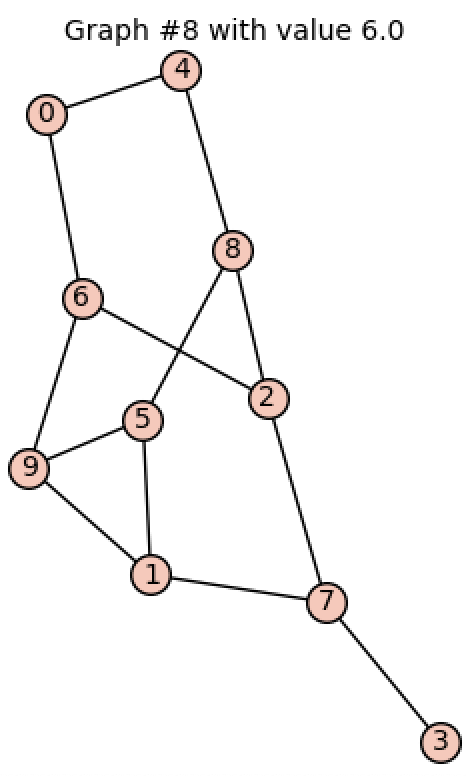
\includegraphics[width=0.2\textwidth]{Images/Screenshot 2025-01-31 at 23.25.16}
    \caption{Graph with PCN 6 on 11 vertices}
    \label{fig:screenshot1}
\end{figure}

\begin{figure}[h]
    \centering
    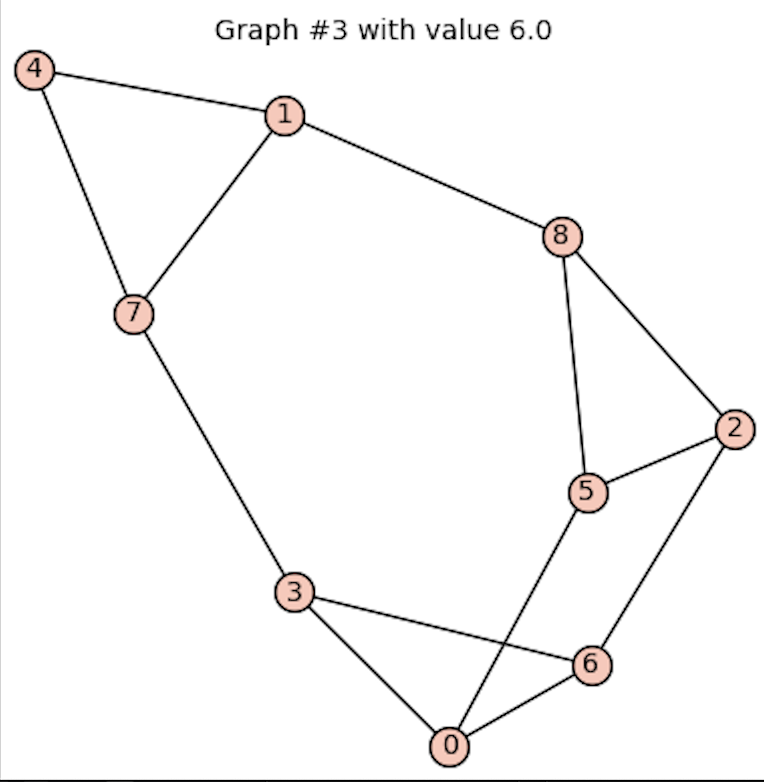
\includegraphics[width=0.2\textwidth]{Images/Screenshot 2025-01-31 at 23.23.59}
    \caption{Graph with PCN 6 on 11 vertices}
    \label{fig:screenshot2}
\end{figure}

\end{document}